% !TEX root = ../../Article.tex
\subsection{Data Transfer Speed}
\paragraph{Description and motivation}\mbox{}\\
%\subsection{Description and Motivation}
Transfer speed is a very vital for part of the smart card interaction. If the smart card application or the transportation layer is incapable of handling large amounts of the data we will need to take that into account when examining the usability of smart cards. In order to test and eliminate as many variables as possible the smart card is programmed to receive data, copy the incoming data to the buffer and send the exact same data in return. Figure \ref{fig:nfcDataflowTest} describes this process using an NFC card as a platform for the Java Card Applet.

\begin{figure}[h!]
  \caption{Data flow of data transfer speed test for NFC.}
  \label{fig:nfcDataflowTest}
  \centering
    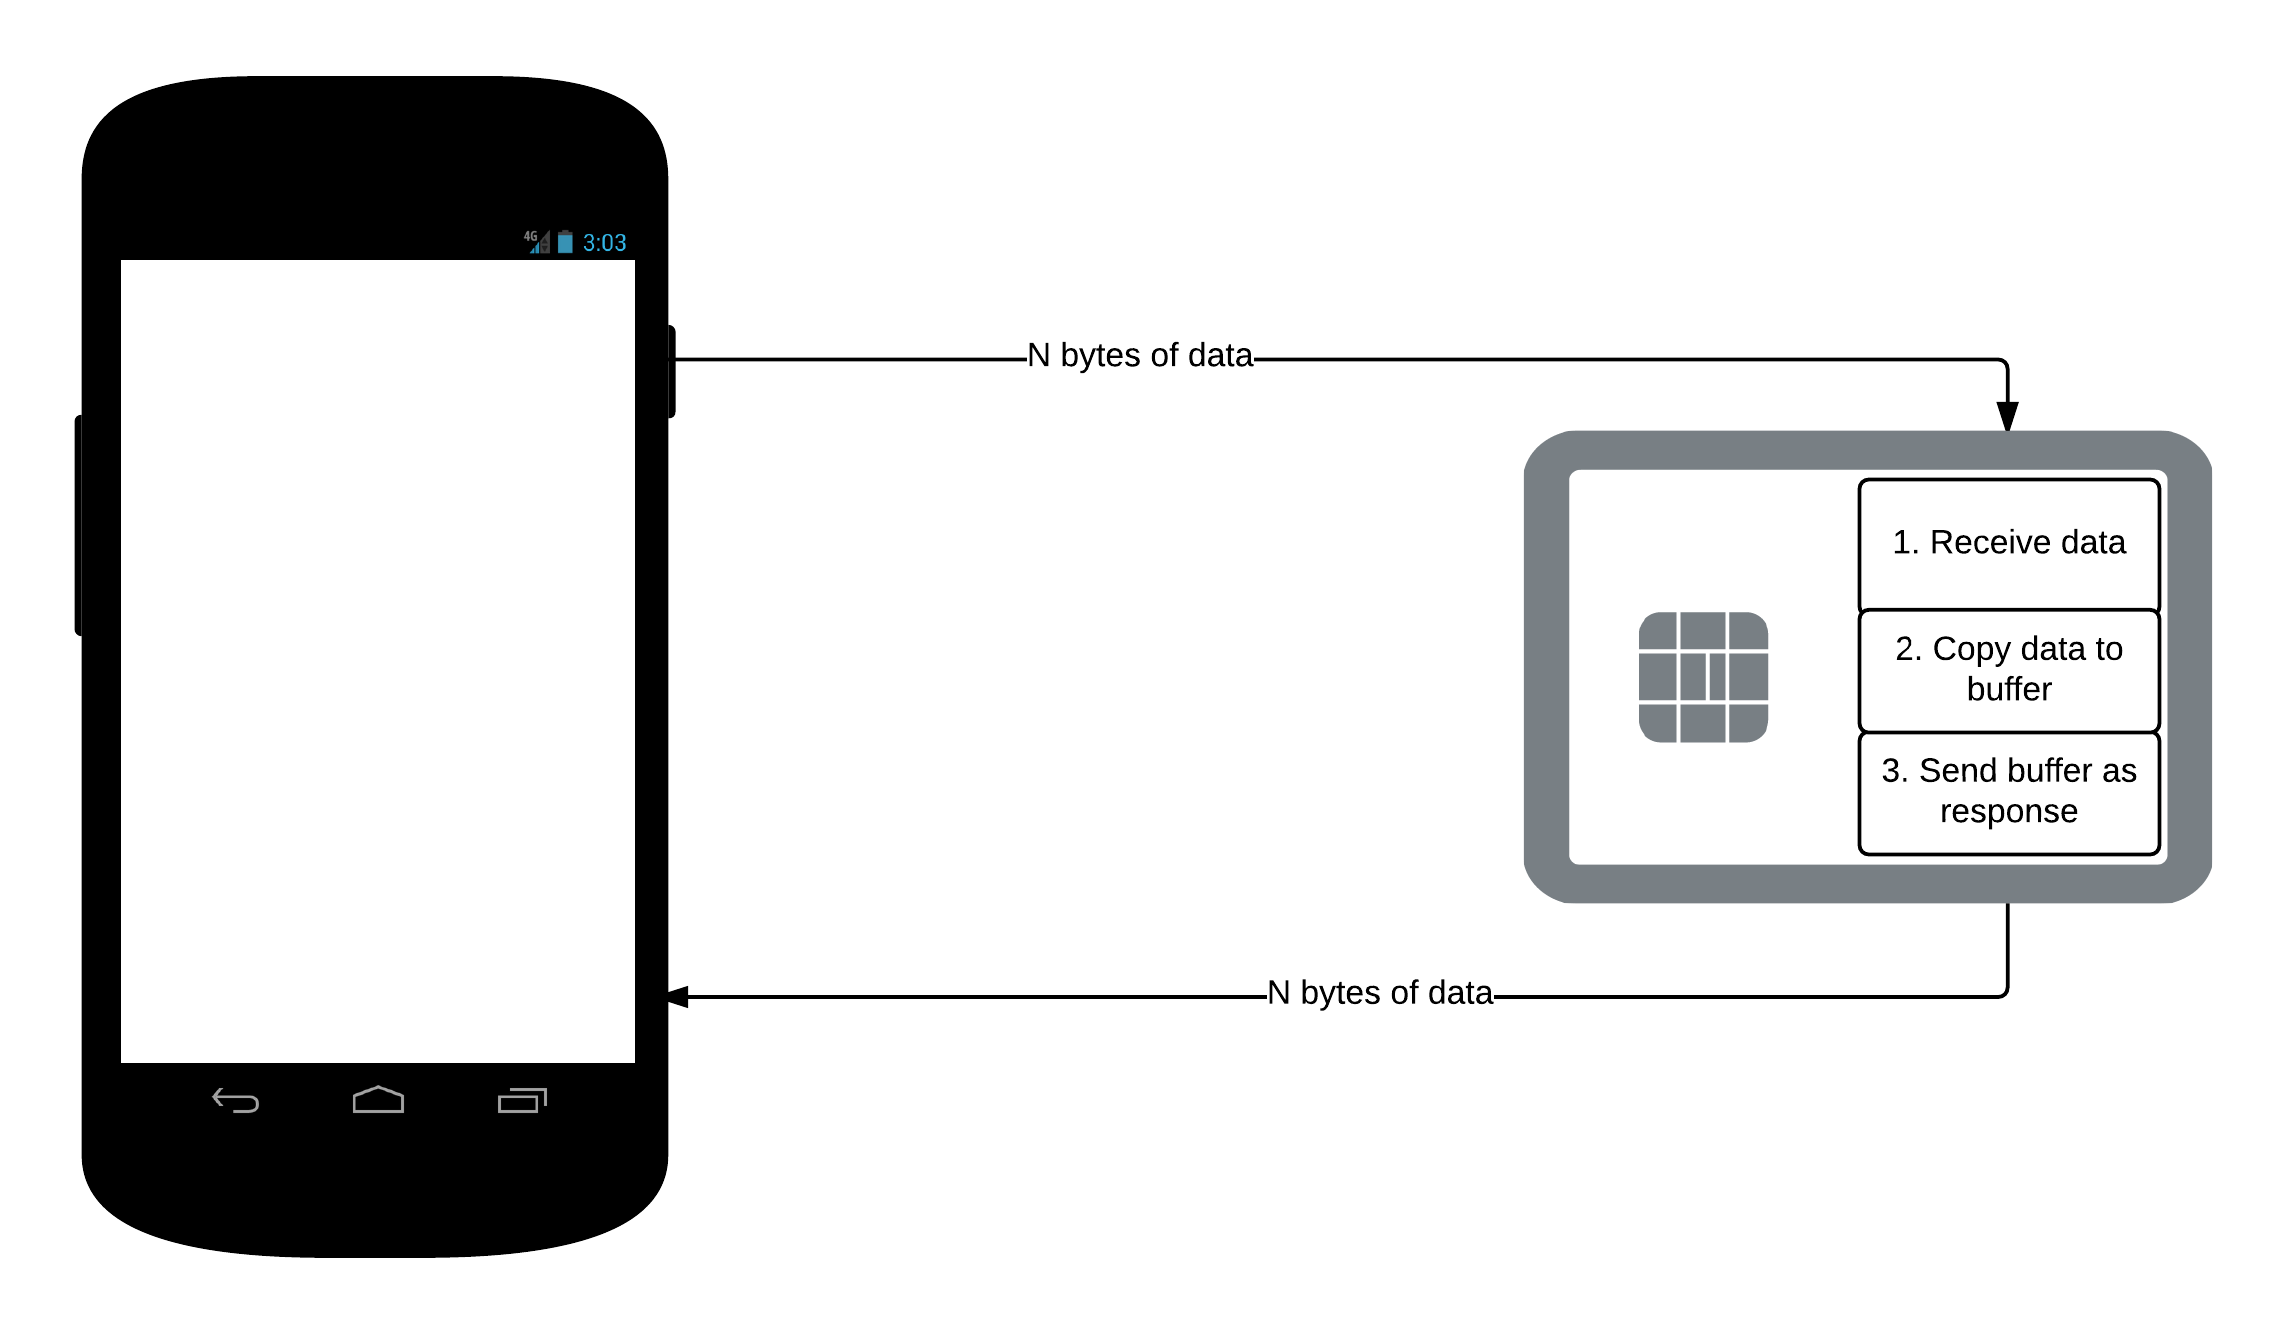
\includegraphics[width=0.95\textwidth]{images/NFCTransferTest.png}
\end{figure}

%\paragraph{Tests and Results}\mbox{}\\
%\subsection{Tests and Results}
%\paragraph{Test setup}\mbox{}\\
The design of the tests was an iterative process. Transfer speed test was one of the first tests we ran on the smart cards and we did not know beforehand how much data a smart card would be able to handle. As a result we ended up with 3 different configurations.

T1 configuration consists of the Android application sending 255 byte of data to the smart card application, receive the response and write the response to an internal file. This process is repeated until all of the data is processed.

T2 configuration consist of the Android application sending data to the smart card application using frames of size 255 byte until all data is sent. Simultaneously the responses are written to an internal file using FileOutputStream (provided by the standard Java library).

T3 configuration consist of the Android application sending data to the smart card application using frames of size 32768 byte until all data is sent. Simultaneously the responses are written to an internal file using FileOutputStream (provided by the standard Java library).

With some pre-testing it quickly became apparent that T1 configuration is vastly inferior to T2 and T3. A non-asynchronous (not using streams) Android application is not representative of the ``real-world'' and we decided on not pursuing further test results using this configuration when we moved over to Micro SD card testing.

\paragraph{NFC results}\mbox{}\\
\begin{table}[h!]
\caption{Table of NFC transfer speed test.}
\label{tbl:nfcspeed}
\centering

    \begin{tabular}{ | l | r | r | r |}
        \hline
        \thead{Data size (byte)}
        & \thead{T1}
        & \thead{T2}
        & \thead{T3} \\ \hline

        10000 & 3,8s & 4,1s & 3,6s \\ \hline
        100000 & 41,3s & 35,0s & 24,7s \\ \hline
        1000000 & 602,1s & 361,3s & 235,1s \\ \hline

    \end{tabular}

\end{table}

%\vspace{1cm}
\begin{figure}[h!]

    \caption{Graphical representation of table \ref{tbl:nfcspeed}.}
    \label{fig:nfcgraph}
    \begin{tikzpicture}
        \centering
            \begin{axis}[
                width  = 0.85*\textwidth,
                height = 8cm,
                major x tick style = transparent,
                ybar=2*\pgflinewidth,
                bar width=14pt,
                ymajorgrids = true,
                ylabel = {Running time (seconds)},
                xlabel = {Data size (byte)},
                symbolic x coords={10000, 100000, 1000000},
                xtick = data,
                scaled y ticks = false,
                enlarge x limits=0.25,
                ymin=0,
                legend cell align=left,
                legend style={
                        at={(1,1.05)},
                        anchor=south east,
                        column sep=1ex
                }
            ]
                \addplot[style={bblue,fill=bblue,mark=none}]
                    coordinates {(10000, 3.89) (100000, 41.29) (1000000, 602)};

                \addplot[style={rred,fill=rred,mark=none}]
                     coordinates {(10000, 4) (100000, 35) (1000000, 361)};

                \addplot[style={ggreen,fill=ggreen,mark=none}]
                     coordinates {(10000, 3.6) (100000, 24) (1000000, 235)};

                \legend{T1 Configuration,T2 Configuration,T3 Configuration}


            \end{axis}
    \end{tikzpicture}
\end{figure}


The tests results(table \ref{tbl:nfcspeed}) show a significant improvement from T1 to T3. The exception is when we are sending small amounts of data to the smart card applet which suggest that the difference is miniscule. However, when we upped the data size to 100.000 byte, T2 and T3 was 15\% and 40\%, respectively, faster than T1. When sending 1.000.000 bytes of data T1 used 602,1s. T2 had an improvement of around 40\% whereas T3 had an improvement of around 60\%. The test results clearly show that T3 is the optimal configuration of the 3.

\newpage
\paragraph{Micro SD results}\mbox{}\\
T1 configuration, from NFC was dropped when testing transfers speed for micro SD as it became clear from previous tests on NFC that T1 is vastly inferior to T2 and T3. A non-asyncronous (not using streams) Android application is not representative of the "real-world" and we decided on not pursuing further test results using this configuration.

T2 configuration consist of the Android application sending data to the smart card application using frames of size 255 byte until all data is sent. Simultaneously the responses are written to an internal file using FileOutputStream (provided by the standard Java library).

We were not able to test T3 configuration as explained in section \ref{sec:limitationsMSD}.

\begin{table}[h!]
\caption{Table of micro SD transfer speed test.}
\label{tbl:msdspeed}
\centering

    \begin{tabular}{ | l | r | r |}
        \hline
        \thead{Data size (byte)}
        & \thead{T2}
        & \thead{T3} \\ \hline

        10000  & 3,18s & N/A s \\ \hline
        100000 & 16,14s & N/A s \\ \hline
        1000000 & 142s & N/A s \\ \hline

    \end{tabular}

\end{table}

As we were not able to test T3 on micro SD cards we cannot compare the configurations with each other. What we can do is compare the T2 results for micro SD to the T2 results from the NFC section. The difference is not that great with small amounts of data, but when we go up to 1.000.000 bytes of data micro SD is 60\% faster than the NFC card (361,3s to 142s). This points in the direction of micro SD cards achieving better results than NFC cards.

\paragraph{Conclusion}\mbox{}\\
%\subsection{Conclusion}
From table \ref{tbl:nfcspeed} and figure \ref{fig:nfcgraph} we can learn that we are able to optimize the data transfer and processing speed between the Android application and the NFC card. It is also clear that when we are transmitting low amounts of data there is virtually no difference between the configurations; T1, T2 and T3. The differences are more prominent when the data amounts increase. Even though we achieved an improvement of approximately 60 \% from T1 to T3 when sending 1 MB of data, the process is still time consuming.

If we compare the test results for T2 configuration on the NFC card and micro SD card we can clearly see an improvement on the micro SD card. The micro SD card had a ~60 \%  better running time over the NFC card when sending 1 MB of data. Although we were not able to test configuration T3 on the micro SD card, results point in the direction of micro SD cards having better performance than NFC cards. We are not able to confirm this and thus cannot be treated as a fact.

Even though we are able to optimize and improve data transfer speeds, we are still very far from transferring and processing large amounts of data quickly. We have to take this into account when evaluating areas of use for the smart card. Transfer and processing speed rules out many areas concerning large amounts of data, such as full data encryption.
